\subsubsection{Auth}

\begin{center}
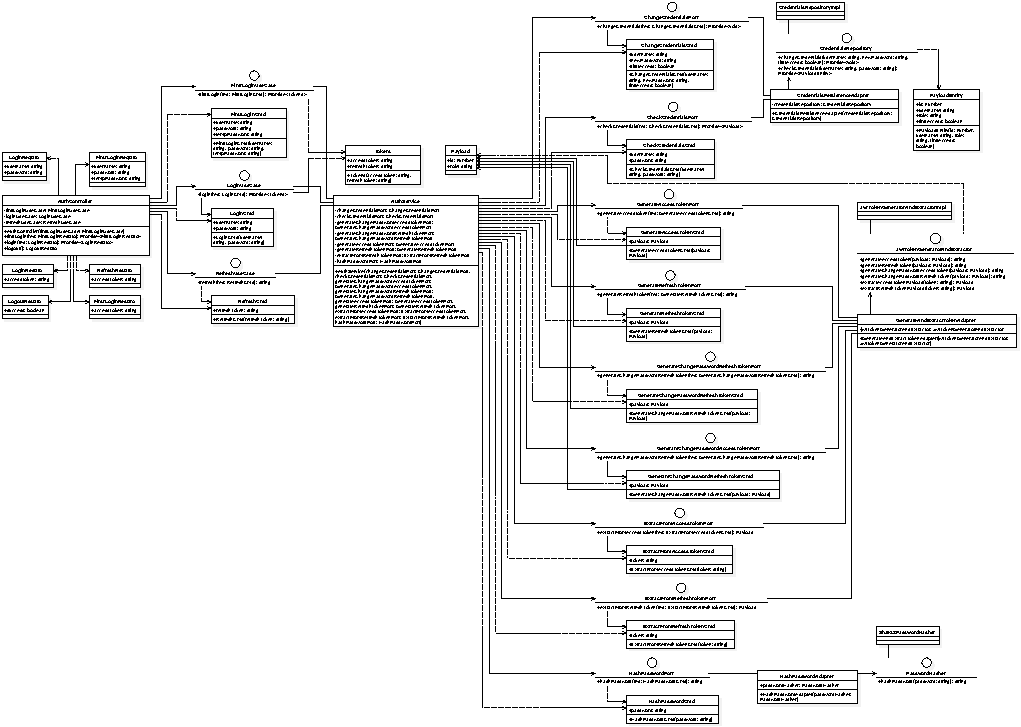
\includegraphics[width=\textwidth]{./backend/auth/auth.pdf}
\captionof{figure}{\href{https://snakebyteteam.github.io/3-PB/Documenti_esterni/Specifica_tecnica/backend/auth/auth.pdf}{Diagramma delle classi del modulo Auth}}
\end{center}

% req

\addAtr{}{username: string}{Username dell'utente che effettua il primo accesso}
\addAtr{}{password: string}{Password temporanea assegnata all'utente}
\addAtr{}{tempPassword: string}{Nuova password scelta dall'utente per sostituire quella temporanea}
\makeCl{FirstLoginReqDto}{DTO di richiesta per il primo accesso, contenente credenziali temporanee e nuova password}

\addAtr{}{username: string}{Username dell'utente}
\addAtr{}{password: string}{Password dell'utente}
\makeCl{LoginReqDto}{DTO di richiesta per l'autenticazione standard}

\addAtr{}{refreshToken: string}{Token di refresh da utilizzare per ottenere un nuovo access token}
\makeCl{RefreshReqDto}{DTO di richiesta per il rinnovo dell'access token}

% res

\addAtr{}{accessToken: string}{Access token generato al termine del primo accesso}
\makeCl{FirstLoginResDto}{DTO di risposta restituito al completamento del primo accesso}

\addAtr{}{accessToken: string}{Access token generato a seguito dell'autenticazione}
\makeCl{LoginResDto}{DTO di risposta restituito a seguito di un'autenticazione avvenuta con successo}

\addAtr{}{success: boolean}{Indica se il logout è avvenuto con successo}
\makeCl{LogoutResDto}{DTO di risposta restituito a seguito di una richiesta di logout}

\addAtr{}{accessToken: string}{Nuovo access token generato a partire dal refresh token}
\makeCl{RefreshResDto}{DTO di risposta restituito a seguito del rinnovo dell'access token}

% model

\addAtr{+}{id: number}{Identificativo univoco dell'utente}
\addAtr{+}{username: string}{Username dell'utente}
\addAtr{+}{role: string}{Ruolo dell'utente nel sistema}
\addAtr{+}{firstAccess: boolean}{Indica se l'utente non ha ancora completato il primo accesso}
\makeCl{Payload}{Modello di dominio che rappresenta il payload contenuto nei token JWT}

\addAtr{+}{accessToken: string}{Token JWT per l'accesso alle risorse protette}
\addAtr{+}{refreshToken: string}{Token JWT per il rinnovo dell'access token}
\makeCl{Tokens}{Modello di dominio che raggruppa la coppia di token JWT generati all'autenticazione}

% controller

\addAtr{-}{firstLoginUseCase: FirstLoginUseCase}{Use case per la gestione del primo accesso}
\addAtr{-}{loginUseCase: LoginUseCase}{Use case per la gestione dell'autenticazione standard}
\addAtr{-}{refreshUseCase: RefreshUseCase}{Use case per il rinnovo dell'access token}
\addMet{+}{firstLogin(req: FirstLoginReqDto): Promise$<$FirstLoginResDto$>$}{Espone l'endpoint per il primo accesso con cambio della password temporanea}
\addMet{+}{login(req: LoginReqDto): Promise$<$LoginResDto$>$}{Espone l'endpoint per l'autenticazione standard con username e password}
\addMet{+}{refresh(req: Request): RefreshResDto}{Espone l'endpoint per il rinnovo dell'access token tramite refresh token}
\addMet{+}{logout(): LogoutResDto}{Espone l'endpoint per l'invalidazione della sessione corrente}
\makeCl{AuthController}{Controller REST che gestisce le richieste HTTP relative all'autenticazione}

% command

\addAtr{+}{username: string}{Username dell'utente di cui aggiornare le credenziali}
\addAtr{+}{newPassword: string}{Nuova password da impostare}
\addAtr{+}{firstAccess: boolean}{Nuovo valore del flag di primo accesso}
\makeCl{ChangeCredentialsCmd}{Comando per l'aggiornamento delle credenziali di un utente}

\addAtr{+}{username: string}{Username da verificare}
\addAtr{+}{password: string}{Password da verificare}
\makeCl{CheckCredentialsCmd}{Comando per la verifica delle credenziali di accesso}

\addAtr{+}{username: string}{Username di cui verificare lo stato di primo accesso}
\makeCl{CheckFirstAccessCmd}{Comando per la verifica se un utente deve ancora completare il primo accesso}

\addAtr{+}{token: string}{Access token da cui estrarre il payload}
\makeCl{ExtractFromAccessTokenCmd}{Comando per l'estrazione del payload da un access token JWT}

\addAtr{+}{token: string}{Refresh token da cui estrarre il payload}
\makeCl{ExtractFromRefreshTokenCmd}{Comando per l'estrazione del payload da un refresh token JWT}

\addAtr{+}{username: string}{Username dell'utente che effettua il primo accesso}
\addAtr{+}{password: string}{Password temporanea dell'utente}
\addAtr{+}{tempPassword: string}{Nuova password scelta dall'utente}
\makeCl{FirstLoginCmd}{Comando per l'esecuzione del flusso di primo accesso}

\addAtr{+}{payload: Payload}{Payload da codificare nell'access token}
\makeCl{GenerateAccessTokenCmd}{Comando per la generazione di un access token JWT standard}

\addAtr{+}{payload: Payload}{Payload da codificare nel token di cambio password}
\makeCl{GenerateChangePasswordAccessTokenCmd}{Comando per la generazione di un access token JWT dedicato al cambio password}

\addAtr{+}{payload: Payload}{Payload da codificare nel refresh token di cambio password}
\makeCl{GenerateChangePasswordRefreshTokenCmd}{Comando per la generazione di un refresh token JWT dedicato al cambio password}

\addAtr{+}{payload: Payload}{Payload da codificare nel refresh token}
\makeCl{GenerateRefreshTokenCmd}{Comando per la generazione di un refresh token JWT standard}

\addAtr{+}{password: string}{Password in chiaro da sottoporre a hashing}
\makeCl{HashPasswordCmd}{Comando per l'hashing sicuro di una password}

\addAtr{+}{username: string}{Username dell'utente che effettua il login}
\addAtr{+}{password: string}{Password dell'utente}
\makeCl{LoginCmd}{Comando per l'esecuzione del flusso di autenticazione standard}

\addAtr{+}{refreshToken: string}{Refresh token da utilizzare per generare un nuovo access token}
\makeCl{RefreshCmd}{Comando per il rinnovo dell'access token tramite refresh token}

% use case

\addMet{+}{firstLogin(req: FirstLoginCmd): Promise$<$Tokens$>$}{Gestisce il primo accesso verificando le credenziali temporanee e aggiornando la password}
\makeItf{FirstLoginUseCase}{Interfaccia del use case per la gestione del primo accesso}

\addMet{+}{login(req: LoginCmd): Promise$<$Tokens$>$}{Verifica le credenziali e genera la coppia di token JWT per la sessione}
\makeItf{LoginUseCase}{Interfaccia del use case per la gestione dell'autenticazione standard}

\addMet{+}{refresh(req: RefreshCmd): string}{Valida il refresh token e genera un nuovo access token}
\makeItf{RefreshUseCase}{Interfaccia del use case per il rinnovo dell'access token}

% service

\addAtr{-}{changeCredentialsPort: ChangeCredentialsPort}{Porta per l'aggiornamento delle credenziali utente}
\addAtr{-}{checkCredentialsPort: CheckCredentialsPort}{Porta per la verifica delle credenziali utente}
\addAtr{-}{generateChangePasswordAccessTokenPort: GenerateChangePasswordAccessTokenPort}{Porta per la generazione dell'access token di cambio password}
\addAtr{-}{generateChangePasswordRefreshTokenPort: GenerateChangePasswordRefreshTokenPort}{Porta per la generazione del refresh token di cambio password}
\addAtr{-}{generateAccessTokenPort: GenerateAccessTokenPort}{Porta per la generazione dell'access token standard}
\addAtr{-}{generateRefreshTokenPort: GenerateRefreshTokenPort}{Porta per la generazione del refresh token standard}
\addAtr{-}{extractFromAccessTokenPort: ExtractFromAccessTokenPort}{Porta per l'estrazione del payload dall'access token}
\addAtr{-}{extractFromRefreshTokenPort: ExtractFromRefreshTokenPort}{Porta per l'estrazione del payload dal refresh token}
\addAtr{-}{hashPasswordPort: HashPasswordPort}{Porta per l'hashing delle password}
\addMet{+}{firstLogin(req: FirstLoginCmd): Promise$<$Tokens$>$}{Implementa il flusso di primo accesso coordinando verifica credenziali, aggiornamento password e generazione token}
\addMet{+}{login(req: LoginCmd): Promise$<$Tokens$>$}{Implementa il flusso di autenticazione standard coordinando verifica credenziali e generazione token}
\makeCl{AuthService}{Servizio applicativo che implementa i use case di autenticazione}

% port

\addMet{+}{changeCredentials(req: ChangeCredentialsCmd): Promise$<$void$>$}{Aggiorna username, password e flag di primo accesso dell'utente nel sistema di persistenza}
\makeItf{ChangeCredentialsPort}{Porta di uscita per l'aggiornamento delle credenziali utente}

\addMet{+}{checkCredentials(req: CheckCredentialsCmd): Promise$<$Payload$>$}{Verifica le credenziali e restituisce il payload dell'utente autenticato}
\makeItf{CheckCredentialsPort}{Porta di uscita per la verifica delle credenziali utente}

\addMet{+}{extractFromAccessToken(req: ExtractFromAccessTokenCmd): Payload}{Decodifica e valida un access token restituendone il payload}
\makeItf{ExtractFromAccessTokenPort}{Porta di uscita per l'estrazione del payload da un access token JWT}

\addMet{+}{extractFromRefreshToken(req: ExtractFromRefreshTokenCmd): Payload}{Decodifica e valida un refresh token restituendone il payload}
\makeItf{ExtractFromRefreshTokenPort}{Porta di uscita per l'estrazione del payload da un refresh token JWT}

\addMet{+}{generateAccessToken(req: GenerateAccessTokenCmd): string}{Genera un access token JWT firmato a partire dal payload fornito}
\makeItf{GenerateAccessTokenPort}{Porta di uscita per la generazione di un access token JWT standard}

\addMet{+}{generateChangePasswordAccessToken(req: GenerateChangePasswordAccessTokenCmd): string}{Genera un access token JWT con scopo limitato al cambio password}
\makeItf{GenerateChangePasswordAccessTokenPort}{Porta di uscita per la generazione di un access token JWT dedicato al cambio password}

\addMet{+}{generateChangePasswordRefreshToken(req: GenerateChangePasswordRefreshTokenCmd): string}{Genera un refresh token JWT con scopo limitato al cambio password}
\makeItf{GenerateChangePasswordRefreshTokenPort}{Porta di uscita per la generazione di un refresh token JWT dedicato al cambio password}

\addMet{+}{generateRefreshToken(req: GenerateRefreshTokenCmd): string}{Genera un refresh token JWT firmato a partire dal payload fornito}
\makeItf{GenerateRefreshTokenPort}{Porta di uscita per la generazione di un refresh token JWT standard}

\addMet{+}{hashPassword(req: HashPasswordCmd): string}{Applica una funzione di hashing alla password e restituisce il digest risultante}
\makeItf{HashPasswordPort}{Porta di uscita per l'hashing sicuro delle password}

% entity

\addAtr{+}{id: number}{Identificativo univoco dell'utente nel database}
\addAtr{+}{username: string}{Username dell'utente}
\addAtr{+}{role: string}{Ruolo dell'utente nel sistema}
\addAtr{+}{firstAccess: boolean}{Indica se l'utente non ha ancora completato il primo accesso}
\makeCl{PayloadEntity}{Entità di persistenza che rappresenta i dati utente estratti dal database per la costruzione del payload JWT}

% adapter

\addMet{+}{hashPassword(req: HashPasswordCmd): string}{Applica l'algoritmo di hashing alla password e restituisce il digest}
\makeCl{HashPasswordAdapter}{Adattatore che implementa la porta di hashing delle password delegando a una libreria crittografica}

\addAtr{-}{credentialsRepository: CredentialsRepository}{Repository per l'accesso alle credenziali utente nel database}
\addMet{+}{changeCredentials(req: ChangeCredentialsCmd): Promise$<$void$>$}{Delega al repository l'aggiornamento delle credenziali dell'utente}
\addMet{+}{checkCredentials(req: CheckCredentialsCmd): Promise$<$Payload$>$}{Delega al repository la verifica delle credenziali e mappa il risultato nel modello di dominio}
\makeCl{CredentialsPersistenceAdapter}{Adattatore di persistenza che implementa le porte relative alle credenziali utente}

\addAtr{-}{jwtTokenGeneratorAndExtractor: JwtTokenGeneratorAndExtractor}{Componente per la generazione e l'estrazione di token JWT}
\addMet{+}{generateRefreshToken(req: GenerateRefreshTokenCmd): string}{Delega al componente JWT la generazione del refresh token standard}
\addMet{+}{generateAccessToken(req: GenerateAccessTokenCmd): string}{Delega al componente JWT la generazione dell'access token standard}
\addMet{+}{generateChangePasswordRefreshToken(req: GenerateChangePasswordRefreshTokenCmd): string}{Delega al componente JWT la generazione del refresh token di cambio password}
\addMet{+}{generateChangePasswordAccessToken(req: GenerateChangePasswordAccessTokenCmd): string}{Delega al componente JWT la generazione dell'access token di cambio password}
\addMet{+}{extractFromAccessToken(req: ExtractFromAccessTokenCmd): Payload}{Delega al componente JWT l'estrazione del payload dall'access token}
\addMet{+}{extractFromRefreshToken(req: ExtractFromRefreshTokenCmd): Payload}{Delega al componente JWT l'estrazione del payload dal refresh token}
\makeCl{GenerateAndExtractTokenAdapter}{Adattatore che implementa le porte di generazione ed estrazione dei token JWT}

% repository

\addMet{+}{checkCredentials(username: string, password: string): Promise$<$PayloadEntity$>$}{Verifica nel database la corrispondenza tra username e password e restituisce i dati dell'utente}
\addMet{+}{changeCredentials(username: string, newPassword: string, \\ firstAccess: boolean): Promise$<$void$>$}{Aggiorna nel database la password e il flag di primo accesso dell'utente specificato}
\makeItf{CredentialsRepository}{Interfaccia del repository per le operazioni di persistenza relative alle credenziali utente}

% token

\addMet{+}{generateAccessToken(payload: Payload): string}{Genera un access token JWT firmato con il payload fornito}
\addMet{+}{generateRefreshToken(payload: Payload): string}{Genera un refresh token JWT firmato con il payload fornito}
\addMet{+}{generateChangePasswordAccessToken(payload: Payload): string}{Genera un access token JWT con scopo limitato al cambio password}
\addMet{+}{generateChangePasswordRefreshToken(payload: Payload): string}{Genera un refresh token JWT con scopo limitato al cambio password}
\addMet{+}{extractAccessTokenPayload(token: string): Payload}{Decodifica e valida un access token restituendone il payload}
\addMet{+}{extractRefreshTokenPayload(token: string): Payload}{Decodifica e valida un refresh token restituendone il payload}
\makeItf{JwtTokenGeneratorAndExtractor}{Interfaccia per la generazione e l'estrazione dei payload dei token JWT}

% password

\addMet{+}{hashPassword(password: string): string}{Applica una funzione di hashing one-way alla password e restituisce il digest risultante}
\makeItf{PasswordHasher}{Interfaccia per l'hashing sicuro delle password}
